\chapter{Developing the Observation Strategy for GOTO}
\label{chap:strategy}
\chaptoc{}

% ########################################

\newpage
\section{Introduction}
\label{sec:strategy_intro}
\begin{colsection}

% ~~~~~~~~~~~~~~~~~~~~

\begin{colsection}

In this chapter I outline my work developing the observing strategy for the GOTO prototype telescope.
\rtxt{Thanks to Darren and Evert <blah><blah><blah>}

\end{colsection}

% ~~~~~~~~~~~~~~~~~~~~

\subsection{GOTO as a survey telescope}
\label{sec:survey_telescope}
% normal mode of operation
% compare to other survey telescopes - ASSASSIN [sic], ZTF
\begin{colsection}

WIP

\end{colsection}

% ~~~~~~~~~~~~~~~~~~~~

\subsection{GOTO as a follow-up telescope}
\label{sec:followup_telescope}
\begin{colsection}

WIP

\end{colsection}

% ~~~~~~~~~~~~~~~~~~~~

\end{colsection}

% ########################################

\newpage
\section{Tiling the sky with GOTO-tile}
\label{sec:gototile}
\begin{colsection}

% ~~~~~~~~~~~~~~~~~~~~

\begin{colsection}

GOTO-tile is a \proglang{Python} module (\pkg{gototile} \rtxt{footnote url?}) created for the \gls{goto} project to contain all the functions and frameworks related to tiling the sky. It was originally developed by Darren White as a way to process \gls{ligo} \gls{gw} skymaps for \gls{goto}, and then maintained by Evert Rol who rearranged it into a module usable for some other telescopes including SuperWASP on La Palma and a proposed southern GOTO node. My contributions to the module have been more fundamental: reworking the foundations to improve how grids are defined and sky maps are applied to them, as well as adding different ways to create skymaps.

\end{colsection}

% ~~~~~~~~~~~~~~~~~~~~

\subsection{Creating sky grids}
\label{sec:grids}
% different ways to make grids
\begin{colsection}

The core of GOTO-tile as it now exists is the \code{SkyGrid} class. This is used to define a sky grid, a collection of `tiles' defined as points on the celestial sphere (Figure~\ref{fig:sphere}). These tiles are aligned to the celestial right ascension/declination coordinates, and are designed to create a base framework for observations to be mapped to.

The most important parameter required when defining a sky grid is the field of view of the telescope, which is taken as the size of the tiles that make up the grid. This is defined by giving a width and height value in degrees, meaning the tiles can only be square or rectangular. This is typically fine for the \gls{goto} array, although there was a period when having three \glspl{ut} in an `L'-shape was considered. This was abandoned due mainly to the complexity of tiling the grid based on abstract shapes.

The second parameter required to define a sky grid is the desired overlap between the tiles. This is given as a value between zero and one in both the right ascension and declination directions, with zero meaning no overlap and one meaning all the tiles are completely overlapping (as this would lead to infinite tiles being created in practice the overlap is restricted to no more than $0.9$). This is used to define the spacing between the tile centrers, although exactly how depends on the algorithm used.

As GOTO-tile has been developed the algorithm used to define tile centres has evolved and improved, but the basic method has remained the same:

\begin{enumerate}
    \item Define equally spaced lines of constant declination, separated by the value $\Delta\delta$ (Figure~\ref{fig:deltadelta}). These lines are the basis for the grid, which is defined in ``strips'' of tiles. Exactly how $\Delta\delta$ is defined based on the field of view and overlap parameters depends on the algorithm, in particular how to deal with the poles in case $\Delta\delta$ is not a factor of \SI{90}{\degree}.
    \item Once the strips are defined, then each is filled equally spaced points separated by the value $\Delta\alpha$ (Figure~\ref{fig:deltaalpha}). This value is constant for each strip but is (in most algorithms) a function of declination ($\Delta\alpha(\delta)$), meaning that moving away from the equator to the poles each strip will contain a reducing number of points.
    \item These points are then defined as the centre of the tiles, the size of which is given by the field of view (Figure~\ref{fig:tiledsphere}).
\end{enumerate}

Once the grid has been created it is encapsulated within the GOTO-tile \code{SkyGrid} class. Each tile is defined by a coordinate at its centre, and each is also given a unique name of the form \code{`T0001'}. The grid itself is also given a name formed using the input field of view and overlap parameters, so a grid created with a field of view of \SI{3.7}{\degree}$\times$\SI{4.9}{\degree} and overlap factor of 0.1 (this is the grid used for the \gls{goto} 4-\gls{ut} all-sky survey) is given the name \code{`allsky-3.7x4.9--0.1--0.1'}. In this way a given tile in a given grid can be recreated just from the names, which is used when storing the grid and tile details in the observation database (see Section~\ref{sec:obsdb}). % chktex 29

% ---------

\begin{figure}[p]
\begin{center}
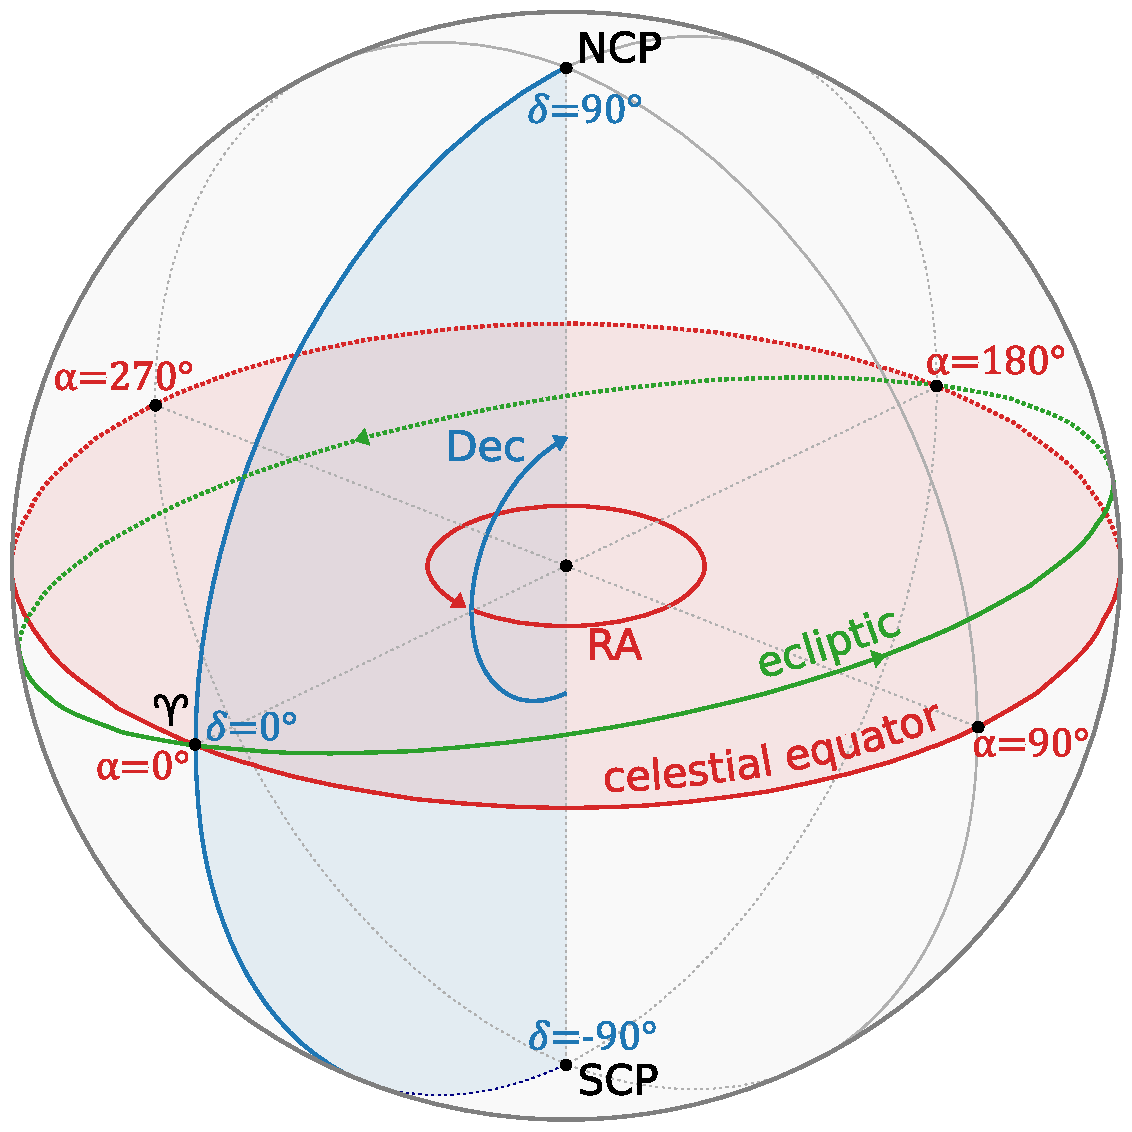
\includegraphics[width=\linewidth]{images/globe1.pdf}
\end{center}
\caption[The celestial sphere]{The celestial sphere. The celestial equator is marked in \textcolor{red}{red}, the vernal equinox (where the ecliptic (not shown) crosses the equator) is marked with the symbol \Aries{} and the meridian that intercepts the vernal equinox is marked in \textcolor{blue}{blue}. The northern and southern celestial poles are marked as NCP and SCP respectively. The definition of the equatorial coordinate system is shown: declination (Dec, $\delta$) is defined as the angle from the equator, ranging from \SI{-90}{\degree} at the SCP to \SI{90}{\degree} at the NCP, and right ascension (RA, $\alpha$) is defined as angle east from the vernal equinox between \SI{0}{\degree} and \SI{360}{\degree}.
}
\label{fig:sphere}
\end{figure}

\begin{figure}[p]
\begin{center}
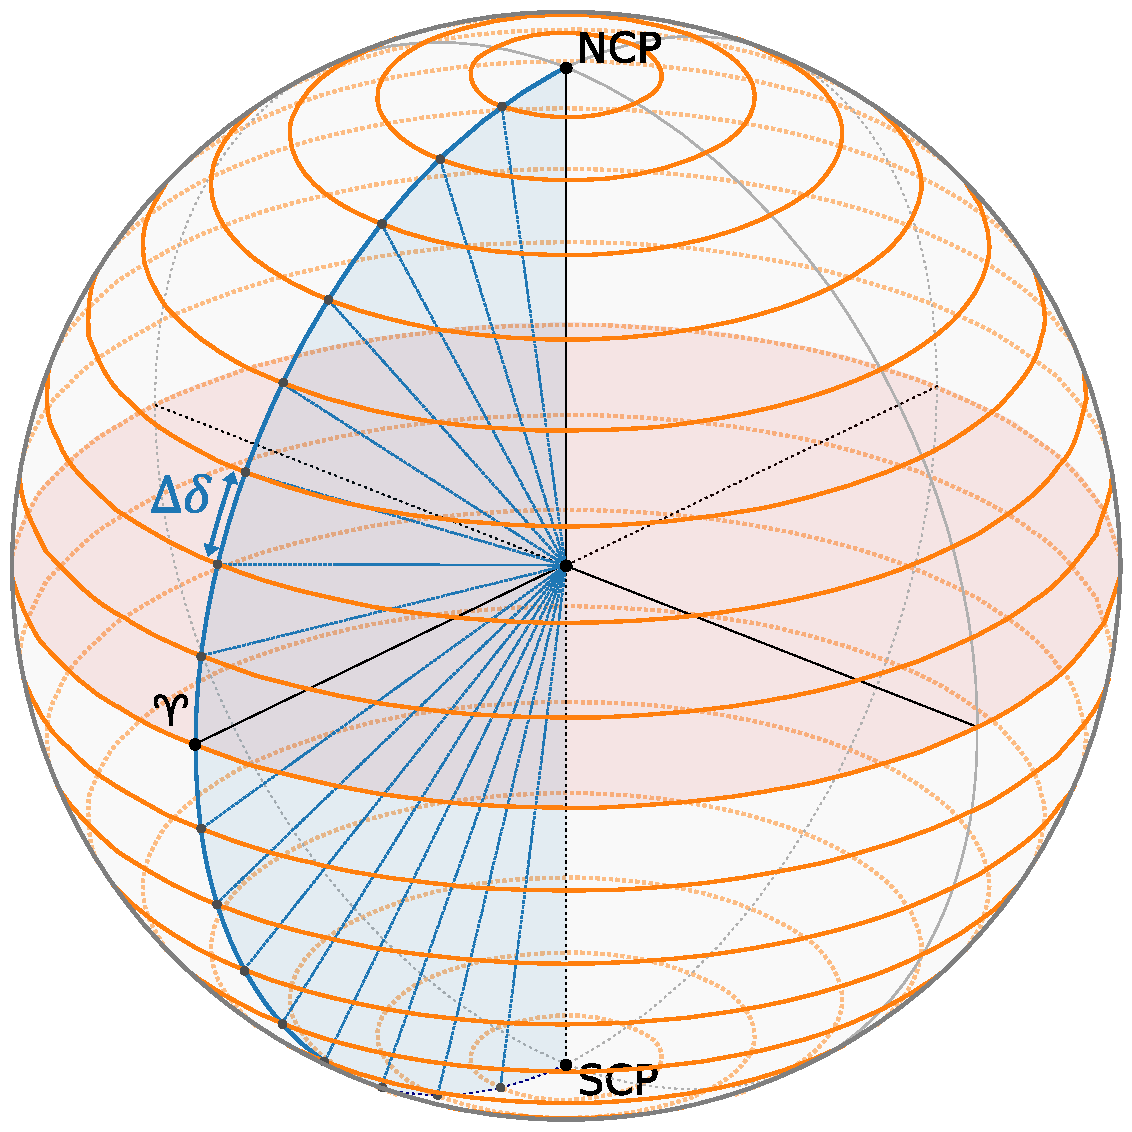
\includegraphics[width=\linewidth]{images/globe2.pdf}
\end{center}
\caption[Defining declination strips]{The first stage when creating a sky grid is defining the declination strips. This is done by dividing the full range of declination (\SI{-90}{\degree} to \SI{90}{\degree}) equally by a constant spacing value $\Delta\delta$. In this example $\Delta\delta =$ \SI{10}{\degree}, and so strips are defined at $\delta=$ \SI{0}{\degree}, \SI{10}{\degree}, \SI{20}{\degree} etc\ldots, and mirrored in the southern hemisphere. There is always a strip with $\delta=0$. Exactly how the strips are defined when $\Delta\delta$ is not an integer factor of \SI{90}{\degree} depends on the algorithm used, in this case using the ``minverlap'' algorithm the strips range from \SI{-90}{\degree} to \SI{90}{\degree} and include a ``strip'' at the poles which will contain single tile (as shown in Figure~\ref{fig:tiledsphere}).
}
\label{fig:deltadelta}
\end{figure}

\begin{figure}[p]
\begin{center}
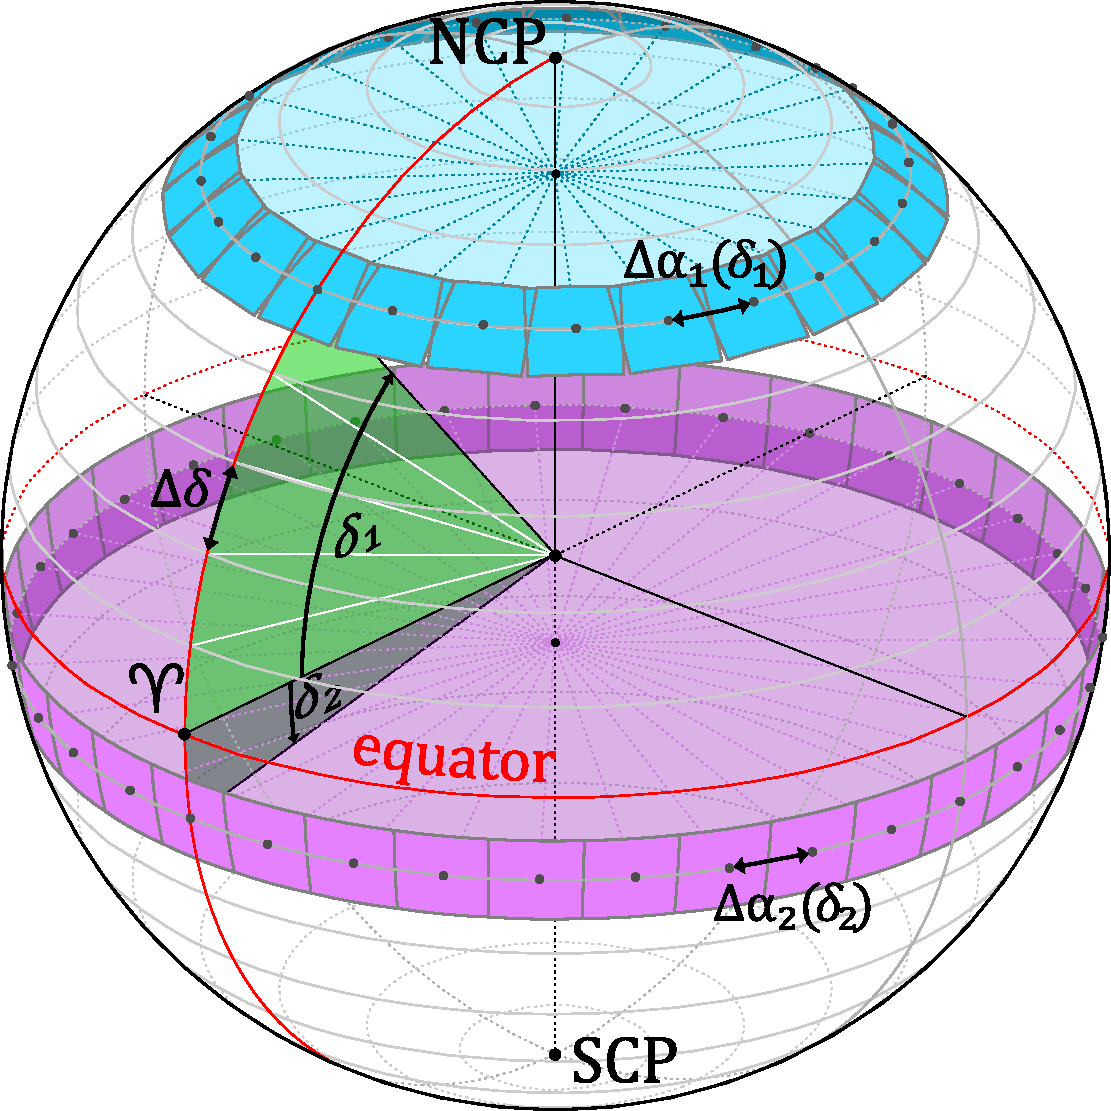
\includegraphics[width=\linewidth]{images/globe3.pdf}
\end{center}
\caption[Defining the spacing between tiles]{After the declination strips are defined (see Figure~\ref{fig:deltadelta}) for each strip tile centres are defined with a set spacing $\Delta\alpha(\delta)$. Unlike $\Delta\delta$, which is fixed across the sphere, $\Delta\alpha$ varies as a function of declination meaning strips closer to the poles will contain fewer tiles. Two examples of defining tiles are shown above, one at declination $\delta_1$ (\SI{50}{\degree}, in \textcolor{cyan}{light blue}) in the northern hemisphere and another at $\delta_2$ (\SI{-10}{\degree}, in \textcolor{Plum}{purple}) in the southern hemisphere. The results of the ``minverlap'' algorithm are shown, previous algorithms had different ways of defining $\Delta\alpha$ that would have resulted in different spacings.
}
\label{fig:deltaalpha}
\end{figure}

\begin{figure}[p]
\begin{center}
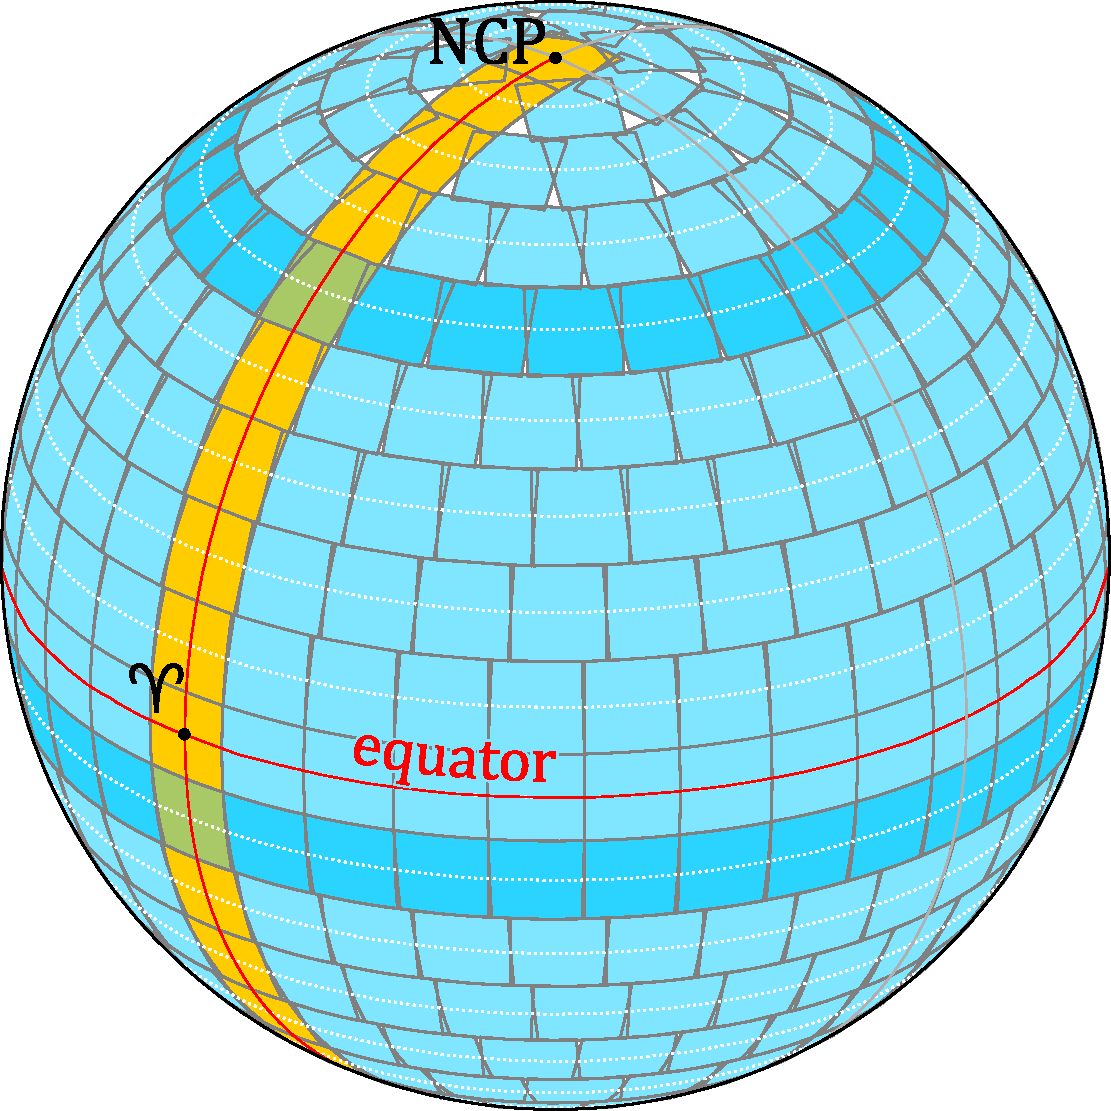
\includegraphics[width=\linewidth]{images/globe4.pdf}
\end{center}
\caption[A fully tiled sphere]{Once every declination strip is complete the full grid is defined, as shown above. The same two strips are shown in \textcolor{cyan}{light blue} and \textcolor{Plum}{purple} as in Figure~\ref{fig:deltaalpha}. Due to each strip starting the tile spacing at RA$=0$, there is a fully aligned column of tiles along the vernal equinox, shown in \textcolor{orange}{yellow}. The grid in these examples was defined using the ``minverlap'' algorithm, with each tile having a field of view of \SI{10}{\degree} $\times$ \SI{10}{\degree} and the overlap was set to zero for clarity (note this leads to gaps between tiles towards the poles). In this case the full grid contains 424 tiles.
\\
}
\label{fig:tiledsphere}
\end{figure}

\newpage

\end{colsection}

% ~~~~~~~~~~~~~~~~~~~~

\subsection{Defining gridding algorithms}
\label{sec:algorithms}
\begin{colsection}

There have been three primary algorithms defined in GOTO-tile's history.

% ---------
\subsubsection{The product algorithm}

The first has since retroactively been called the ``\textbf{product}'' algorithm, and was used when Darren White first wrote GOTO-tile. It first defines the declination step size as

\begin{equation}
    \Delta\delta = f_\text{dec}(1-v_\text{dec}),
    \label{eq:product_deltadelta}
\end{equation}

where $f_\text{dec}$ and $v_\text{dec}$ are respectively the field of view and overlap parameters in the declination direction. The declination strips are then defined by taking steps of this size from the equator towards the poles, stopping when $|\delta| > 90$. The equivalent formula is used to calculate the steps in right ascension

\begin{equation}
    \Delta\alpha = f_\text{RA}(1-v_\text{RA}).
    \label{eq:product_deltaalpha}
\end{equation}

The clear downside of this method is that $\Delta\alpha$ does not vary depending on declination. In effect this algorithm attempts to define the grid as if it was on a flat plane, where the tiles could be arranged in orthogonal rows and columns. In practice when applied to a sphere this leads to a vast number of redundant tiles at the poles, as shown in Figure~\ref{fig:product}.

% ---------
\subsubsection{The cosine algorithm}

Due to the obvious problems with the previous algorithm a replacement was written by Evert Rol, which I have since called the ``\textbf{cosine}'' algorithm. It is a more refined version of the ``product'' algorithm, and the declination strips are calculated in the same manor using Equation~(\ref{eq:product_deltadelta}). However Equation~(\ref{eq:product_deltaalpha}) is modified to depend on declination into

\begin{equation}
    \Delta\alpha(\delta) = \frac{f_\text{RA}(1-v_\text{RA})}{\cos(\delta)}.
    \label{eq:cosine_deltaalpha}
\end{equation}

This produces a much more sensible grid as shown in Figure~\ref{fig:cosine}. However there remained an issue of asymmetry: the strips are arranged increasing and decreasing from $\delta=0$ and the tiles are then arranged within the strips starting from $\alpha=0$. As visible in Figure~\ref{fig:cosine} this leads to varying overlaps when the the tiles within the strips overlap as $\alpha$ approaches \SI{360}{\degree}. Although more subtle there are similar issues at the north and south poles, and it's common for there to be small gaps between the tiles at high and low declinations.

% ---------
\subsubsection{The minverlap algorithm}

Due to these problems I created a new method to create the grid, called the ``\textbf{minverlap}'' (minimum overlap) algorithm. The same grid created with this algorithm is shown in Figure~\ref{fig:minverlap}. The intention of the new algorithm was to solve these issues by adjusting the spacing between tiles to prevent odd gaps. The previous two algorithms both treat the given overlap parameter as as unegotiable, and if the resulting spacings don't give an integer number of tiles within the ranges available then there are uneven gaps at the edges. This is shown more clearly in Figure~\ref{fig:cosine_spacing}, where a tricky spacing results in gaps at the poles and variable overlaps on the meridian. The ``minverlap'' algorithm solves this by treating the given overlap parameter not as fixed but as the \textit{minimum} required overlap between tiles. If a grid is requested with an overlap of $0.2$ (20\%), but the odd field of view of the tiles doesn't fit neatly into the ranges then the overlap can be incensed until the tiles fit.

In order to do this mathematically, it is first necessary to find the number of tiles $n$ that would fit into the range using the previous spacing, and then if it isn't an integer number round it up to the next whole number. In declination this is calculated as

\begin{equation}
    n_\text{dec} = \left \lceil \frac{90}{f_\text{dec}(1-v_\text{dec})} \right \rceil,
    \label{eq:minverlap_ndec}
\end{equation}

where $\lceil x \rceil$ is the mathematical ceiling function. This is a modification of the previous Equation~(\ref{eq:product_deltadelta}) but one that will always find an integer number of tiles. For example, with $f_\text{dec} = $ \SI{13}{\degree} and $v_\text{dec} = 0.2$ the previous spacing $\Delta\delta = 13 \times (1-0.2) = $ \SI{10.4}{\degree}. This clearly doesn't divide into the \SI{90}{\degree} range without a remainder, which is \SI{6.8}{\degree} as shown in Figure~\ref{fig:cosine_spacing}. The problem is that \SI{90}{\degree} $/$ \SI{10.4}{\degree} $= 8.65$. So the previous algorithms will fit in 8 tiles and have over half a tile remaining at the poles. Instead the minverlap algorithm rounds this up to $n_\text{dec} = 9$ tiles, and then simply calculates the spacing using

\begin{equation}
    \Delta\delta = \frac{90}{n_\text{dec}}.
    \label{eq:minverlap_deltadelta}
\end{equation}

In this case the new $\Delta\delta = $ \SI{10}{\degree}, which gives an even arrangement of tiles from the equator to the poles, as shown in Figure~\ref{fig:minverlap_spacing}. The other benefit of this method is that, in addition to there always being a declination strip at $\delta=0$, there will always be ``strips'' at \SI{+90}{\degree} and \SI{-90}{\degree}, which results in a single tile being located covering the poles and ensuring there are no major gaps in coverage.

Right ascension is treated similarly. The integer number of tiles that can fit into a given declination strip is given by

\begin{equation}
    n_\text{RA}(\delta) = \left \lceil \frac{360}{f_\text{RA}(1-v_\text{RA})/\cos(\delta)} \right \rceil + 1,
    \label{eq:minverlap_nra}
\end{equation}

where the $+1$ is here necessary to account for tiles being located both at $\alpha=$\SI{0}{\degree} and $\alpha=$\SI{360}{\degree}. The logic is exactly the same as with declination, and the revised spacing is given by

\begin{equation}
    \Delta\alpha(\delta) = \frac{360}{n_\text{RA}(\delta)}.
    \label{eq:minverlap_deltaalpha}
\end{equation}

The effect of this is also shown in Figure~\ref{fig:minverlap_spacing}, and tiles are uniformly spaced around the declination strip. Note here the ceiling function does produce a slight degeneracy in $\Delta\alpha$ being a function of $\delta$. Using the same parameters as the previous example $\Delta\delta=$\SI{10}{\degree}, so declination strips start at \SI{0}{\degree} and continue to \SI{\pm10}{\degree}, \SI{\pm20}{\degree} \ldots (mirrored in both hemispheres). From Equation~(\ref{eq:minverlap_nra}) the number of tiles on the equator is $n_\text{RA}(\delta=\SI{0}{\degree}) = \lceil 360/(10.4/\cos(0)) \rceil + 1 = \lceil 34.6 \rceil + 1 = 36$. But on the next strip up (or down) $n_\text{RA}(\delta=\SI{\pm10}{\degree}) = \lceil 360/(10.4/\cos(\pm10)) \rceil + 1 = \lceil 34.1 \rceil + 1 = 36$ as well. This is a natural occurrence as there are only a limited number of ways to fit an integer number of fixed tiles into a given range, and so as shown in Figure~\ref{fig:minverlap} the three strips around the equator align perfectly with the same number of tiles.

% ---------
\subsubsection{Limitations of the minverlap algorithm}

The new ``minverlap'' algorithm is an improvement on the previous versions, in particular as it reduces the occurrences of gaps in coverage closer to the poles that happened when using the ``cosine'' algorithm. However the new algorithm is not perfect and gaps can still occur if the starting overlap parameter is very low. For example, Figure~\ref{fig:tiledsphere} shows a sphere tiled using the ``minverlap'' algorithm and an overlap parameter of 0. In this case gaps are visible in the strips of tiles just below the northern celestial pole. A proposed solution to this problem would be to force tiles to meet at their lower corners (in the northern hemisphere, upper corners in the south), therefore overlapping further and removing the possibility of gaps forming due to the angle between the tiles. An attempt to make this change and create an ``enhanced minverlap'' algorithm was tested, however ultimately it proved unnecessary. Although the current algorithm is deficient at low overlap values, this is only an issue for large tiles and very low overlaps. The \SI{10}{\degree} $\times$ \SI{10}{\degree} tiles and 0\% overlap used for Figure~\ref{fig:tiledsphere} are extreme values, and even for the roughly \SI{8}{\degree} $\times$ \SI{5}{\degree} full field of view of a full GOTO telescope the overlap has to be less than 10\% before noticeable gaps start appearing. As well, from the site on La Palma the northern celestial pole is actually below \glspl{goto} nominal horizon of \SI{30}{\degree}, therefore meaning tiles close to the pole will never be visible and the gaps in coverage were irrelevant. Should GOTO-tile be applied in the future to other projects then this issue would need to be revisited, but it was not a priority to fix within the context of this work.

% ---------

\begin{figure}[p]
\begin{minipage}[c]{0.46\textwidth}
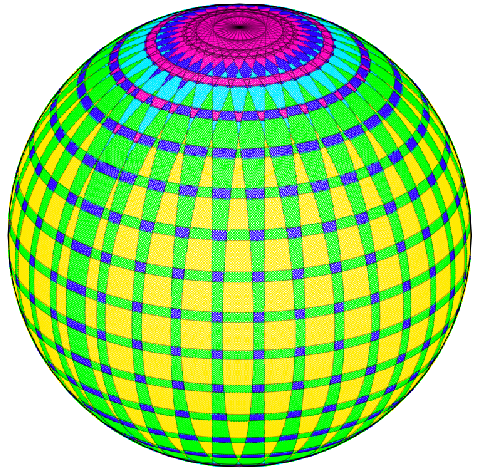
\includegraphics[width=\linewidth]{images/algo_product.pdf}
\end{minipage}
\hfill
\begin{minipage}[c]{0.50\textwidth}
\caption[The ``product'' gridding algorithm]{A sky grid of tiles defined using the ``product'' gridding algorithm. The inputs were a field of view of \SI{13}{\degree} $\times$ \SI{13}{\degree} and an overlap factor of $0.2$ in both axes. The colours show overlapping coverage: \textcolor{Yellow}{yellow} areas are within only one tile, \textcolor{green}{green} two, \textcolor{blue}{blue} three, \textcolor{cyan}{cyan} four and \textcolor{RubineRed}{pink} five or more. This grid contains 595 tiles. Note the constant spacing of tiles in RA and the huge number of redundant tiles at the pole.}
\label{fig:product}
\end{minipage}
\end{figure}

\begin{figure}[p]
\begin{minipage}[c]{0.50\textwidth}
\caption[The ``cosine'' gridding algorithm]{A sky grid of tiles defined using the ``product'' gridding algorithm. The input parameters and colours are the same as in Figure~\ref{fig:product}. This grid contains 393 tiles. Note the asymmetric ``seam'' along the $\alpha=0$ meridian, and the \textcolor{red}{red} areas near the pole that are not within the area of any tiles.}
\label{fig:cosine}
\end{minipage}
\hfill
\begin{minipage}[c]{0.46\textwidth}
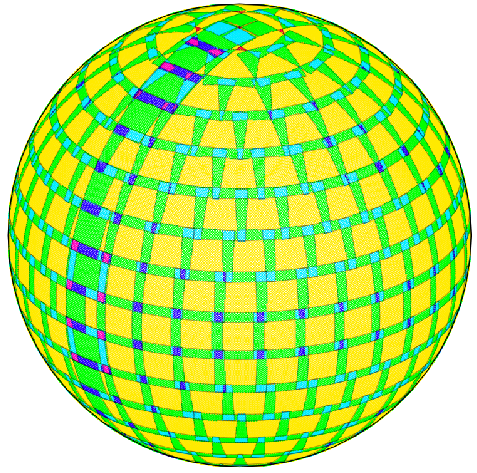
\includegraphics[width=\linewidth]{images/algo_cosine.pdf}
\end{minipage}
\end{figure}

\begin{figure}[p]
\begin{minipage}[c]{0.46\textwidth}
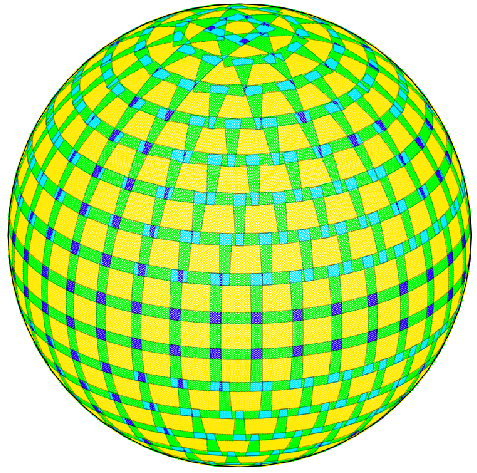
\includegraphics[width=\linewidth]{images/algo_minverlap.pdf}
\end{minipage}
\hfill
\begin{minipage}[c]{0.50\textwidth}
\caption[The ``minverlap'' gridding algorithm]{A sky grid of tiles defined using the ``minverlap'' gridding algorithm. The input parameters and colours are the same as in Figure~\ref{fig:product}. This grid contains 407 tiles.  Note the even spacing of tiles even over the $\alpha=0$ meridian, and the better coverage at the pole.}
\label{fig:minverlap}
\end{minipage}
\end{figure}

% ---------

\begin{figure}[p]
\begin{center}
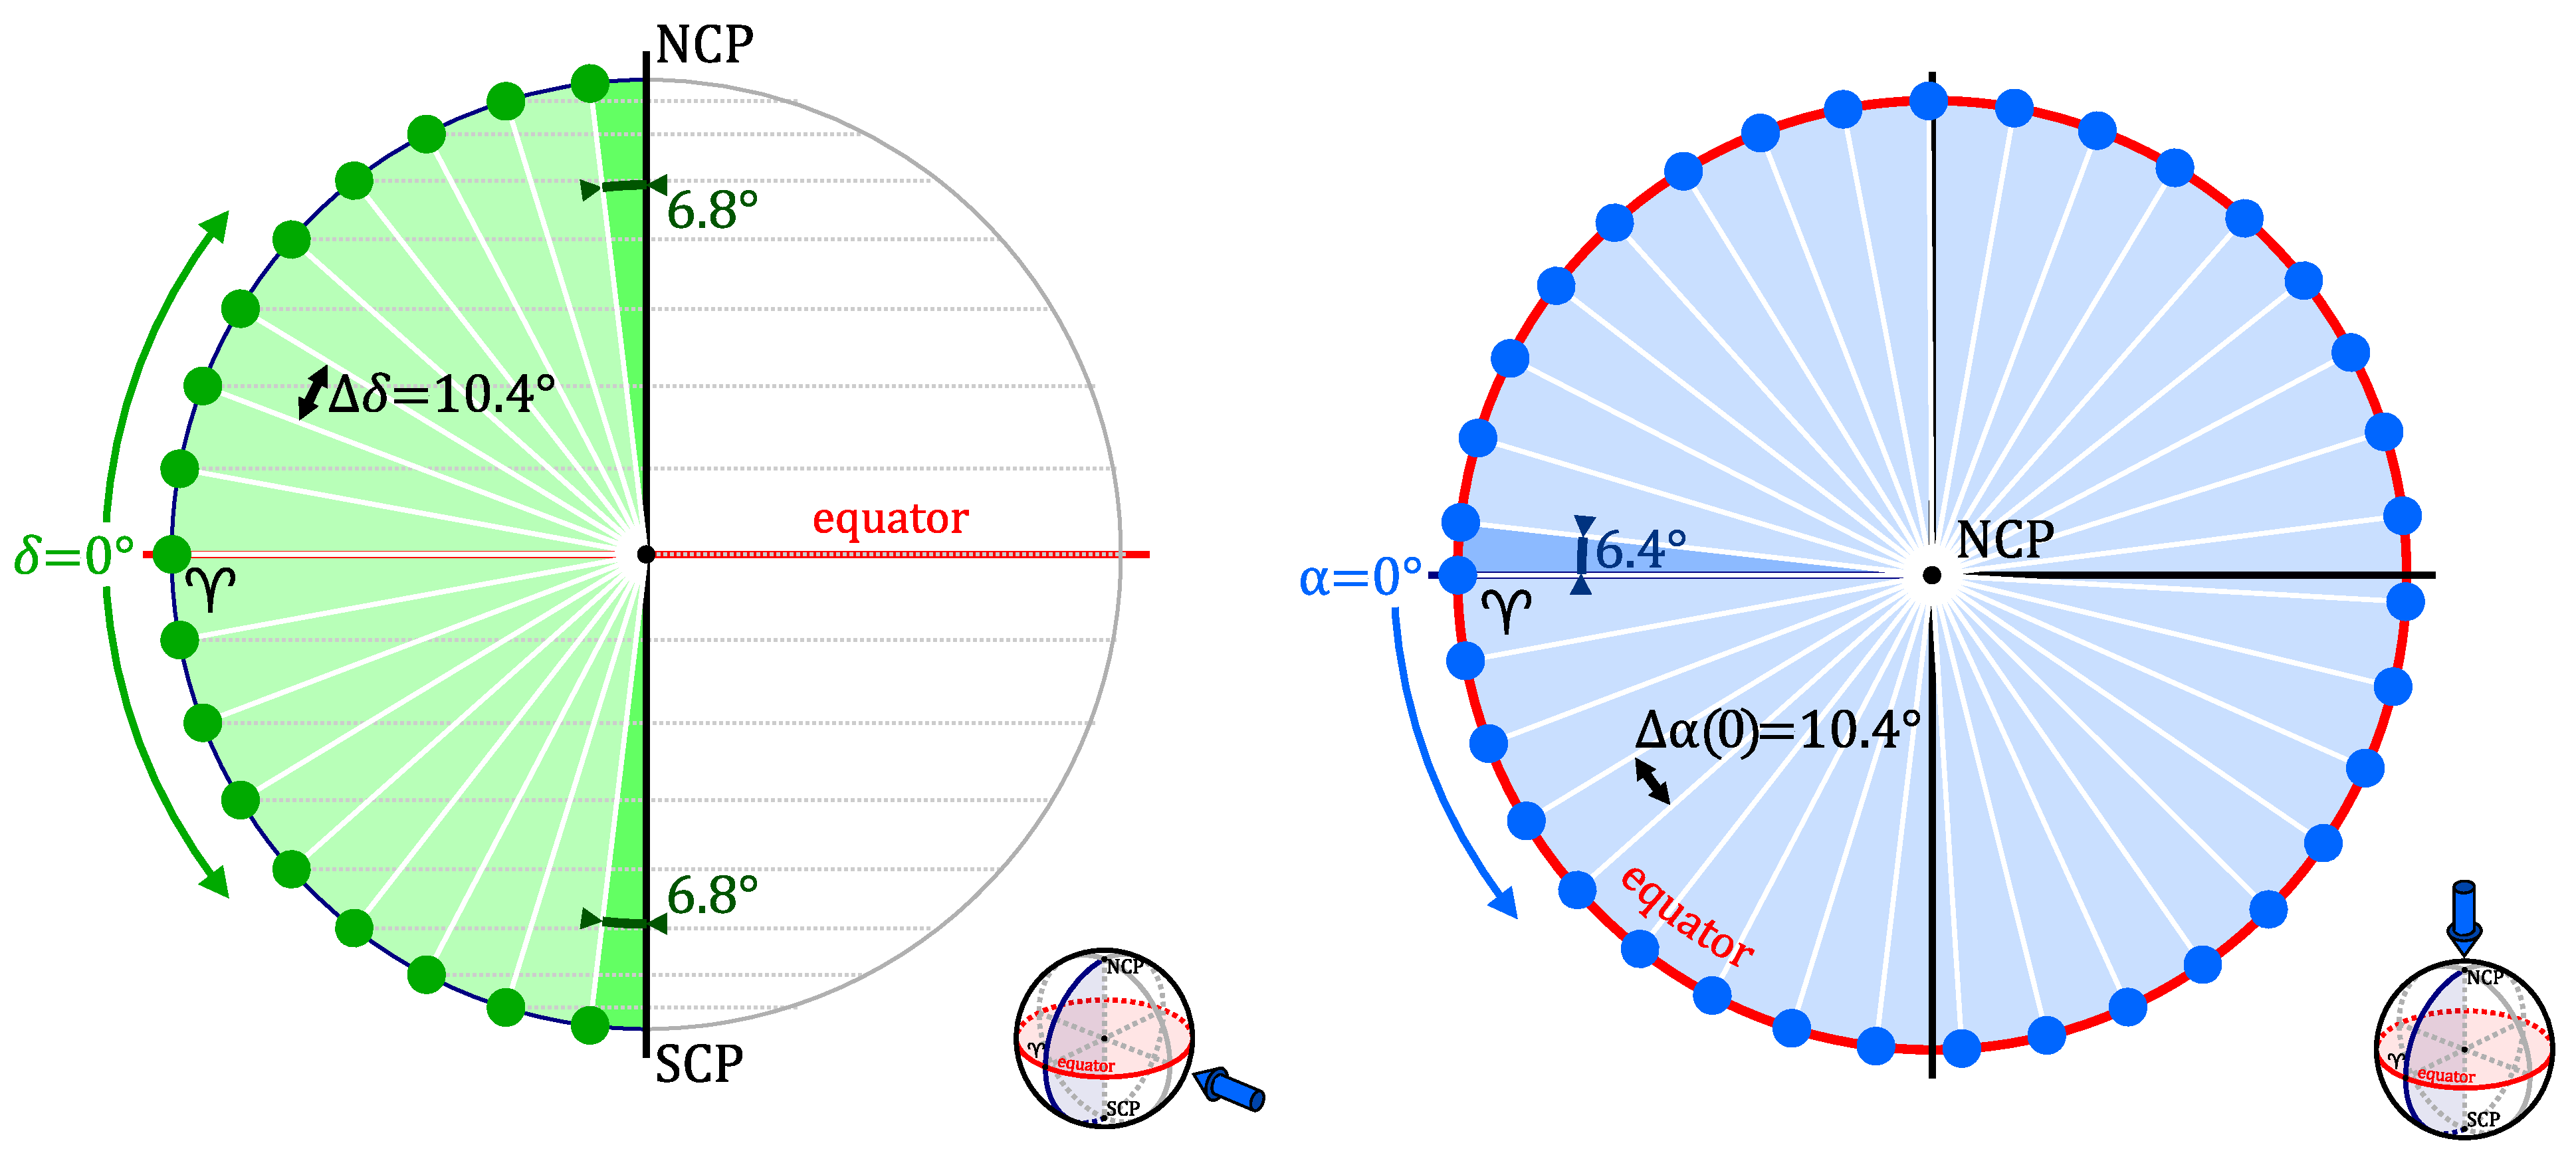
\includegraphics[width=\linewidth]{images/spacing_cosine.pdf}
\end{center}
\caption[Tile spacing with the ``cosine'' algorithm]{Tile spacing with the ``cosine'' algorithm, with a \SI{13}{\degree}$\times$\SI{13}{\degree} FoV and $0.2$ overlap.
\\
\textbf{Left}: Equation~\ref{eq:product_deltadelta} gives $\Delta\delta = $ \SI{10.4}{\degree}, which does not divide into \SI{90}{\degree} without a remainder. 17 strips are defined moving away from $\delta=0$, with last being \SI{6.8}{\degree} from the poles. As this is less than half of the field of view (\SI{6.5}{\degree}) the poles themselves will not fall within the area of any tile.
\\
\textbf{Right}: Equation~\ref{eq:cosine_deltaalpha} gives $\Delta\alpha = $ \SI{10.4}{\degree} on the equator ($\delta=0$). This results in 35 tiles and a reduced spacing of \SI{6.4}{\degree} to the west of the $\alpha=0$ meridian. This remainder will be different for each strip as $\delta$ changes, as visible in Figure~\ref{fig:cosine}.
}
\label{fig:cosine_spacing}
\end{figure}

\begin{figure}[p]
\begin{center}
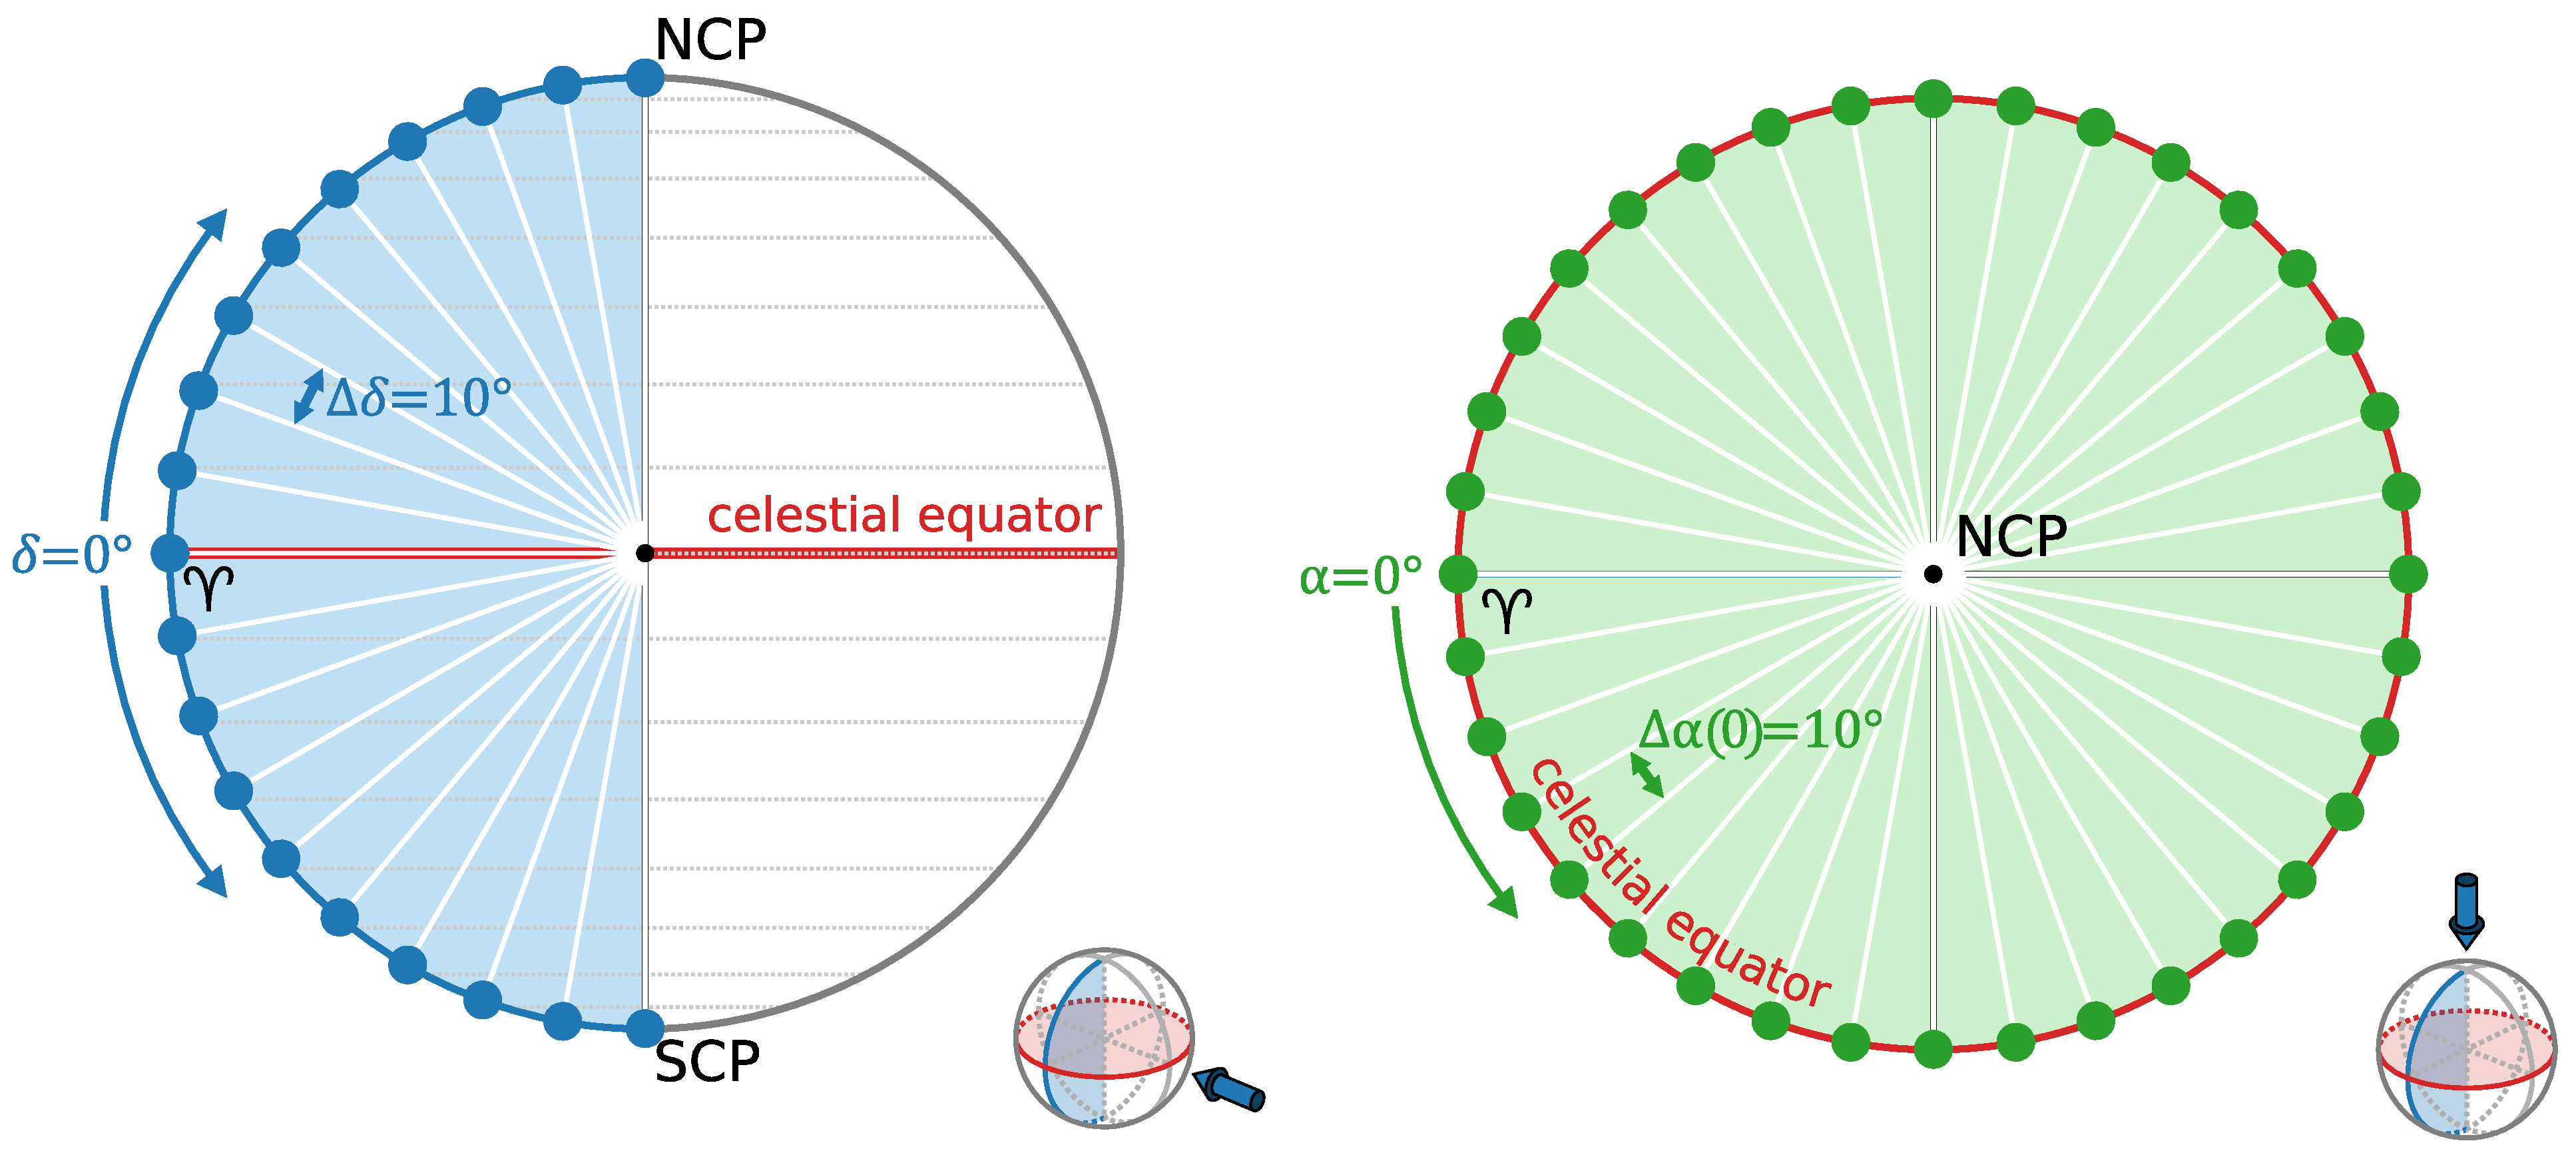
\includegraphics[width=\linewidth]{images/spacing_minverlap.pdf}
\end{center}
\caption[Tile spacing with the ``minverlap'' algorithm]{Tile spacing with the ``minverlap'' algorithm, with the same parameters as Figure~\ref{fig:cosine_spacing}.
\\
\textbf{Left:} Equation~\ref{eq:minverlap_deltadelta} gives $\Delta\delta = $ \SI{10}{\degree}, therefore neatly arranging 19 strips between \SI{-90}{\degree} and \SI{90}{\degree}.
\\
\textbf{Right:} Equation~\ref{eq:minverlap_deltaalpha} also gives $\Delta\alpha = $ \SI{10}{\degree} on the equator ($\delta=0$), so 36 tiles are uniformly arranged around the circumference of the sphere.
}
\label{fig:minverlap_spacing}
\end{figure}

\newpage

\end{colsection}

% ~~~~~~~~~~~~~~~~~~~~

\subsection{HEALPix and probability sky maps}
\label{sec:skymaps}
\begin{colsection}

\gls{healpix} is a system used to define pixelised data on the surface of a sphere~\citep{HEALPix}. Developed at NASA JPL for microwave background data, it is now widely used for other applications including for gravitational wave skymaps produced by the \gls{lvc}. HEALPix divides the sphere into a series of nested (hierarchical) equal-area (although not equal-shape) pixels arranged in declination strips (``isoLatitude''). Shown in Figure~\ref{fig:healpix} are the first four orders of spheres, starting from a base resolution with 12 pixels and increasing as each pixel is split into four. The resolution of the sphere is defined using the $N_\text{side}$ parameter, which is given by the number of pixels along the side of one of the 12 base pixels in the given resolution. At every resolution each base-resolution pixel contains $N_\text{side}^2$ pixels, so the total number of pixels in a sphere is given by

\begin{equation}
    N_\text{pix} = 12 N_\text{side}^2.
    \label{eq:healpix_npix}
\end{equation}

Each pixel therefore has an equal area of

\begin{equation}
    \Omega_\text{pix} = \frac{4\pi}{12 N_\text{side}^2} = \frac{\pi}{3 N_\text{side}^2},
    \label{eq:healpix_area}
\end{equation}

on a unit sphere where the radius $r=1$. Taking the celestial sphere, the circumference in degrees is $\SI{360}{\degree} = 2 \pi r$ meaning the area of the whole sky is given by

\begin{equation}
    A_\text{sky} = 4 \pi r^2 = 4 \pi \left ( \frac{\SI{360}{\degree}}{2 \pi} \right )^2 = \frac{129600}{\pi}~\text{sq deg} \approx 41252~\text{sq deg} , %chktex 3
    \label{eq:sky_area}
\end{equation}

and therefore the area of each HEALPix pixel is

\begin{equation}
    A_\text{pix} = \frac{129600}{12 \pi N_\text{side}^2}~\text{sq~deg} \approx \frac{3438}{N_\text{side}^2}~\text{sq~deg}.
    \label{eq:healpix_area_degrees}
\end{equation}

Figure~\ref{fig:healpix} shows only the first four orders of HEALPix pixelisation, up to $N_\text{side} = 8$ where the sphere is split into 768 pixels each with an area (which can be considered the resolution of the grid) of 53.7~sq deg. An initial, low-resolution \gls{lvc} skymap might use a grid with $N_\text{side} = 64$ (49 thousand pixels) and resolution (pixel area) of 0.84~sq~deg, where as a final output skymap will have $N_\text{side} = 1024$, 12.5 million pixels and a resolution of $3.27 \times 10^{-3}$~sq~deg (11.7 square arcminutes).

\begin{figure}[t]
\begin{center}
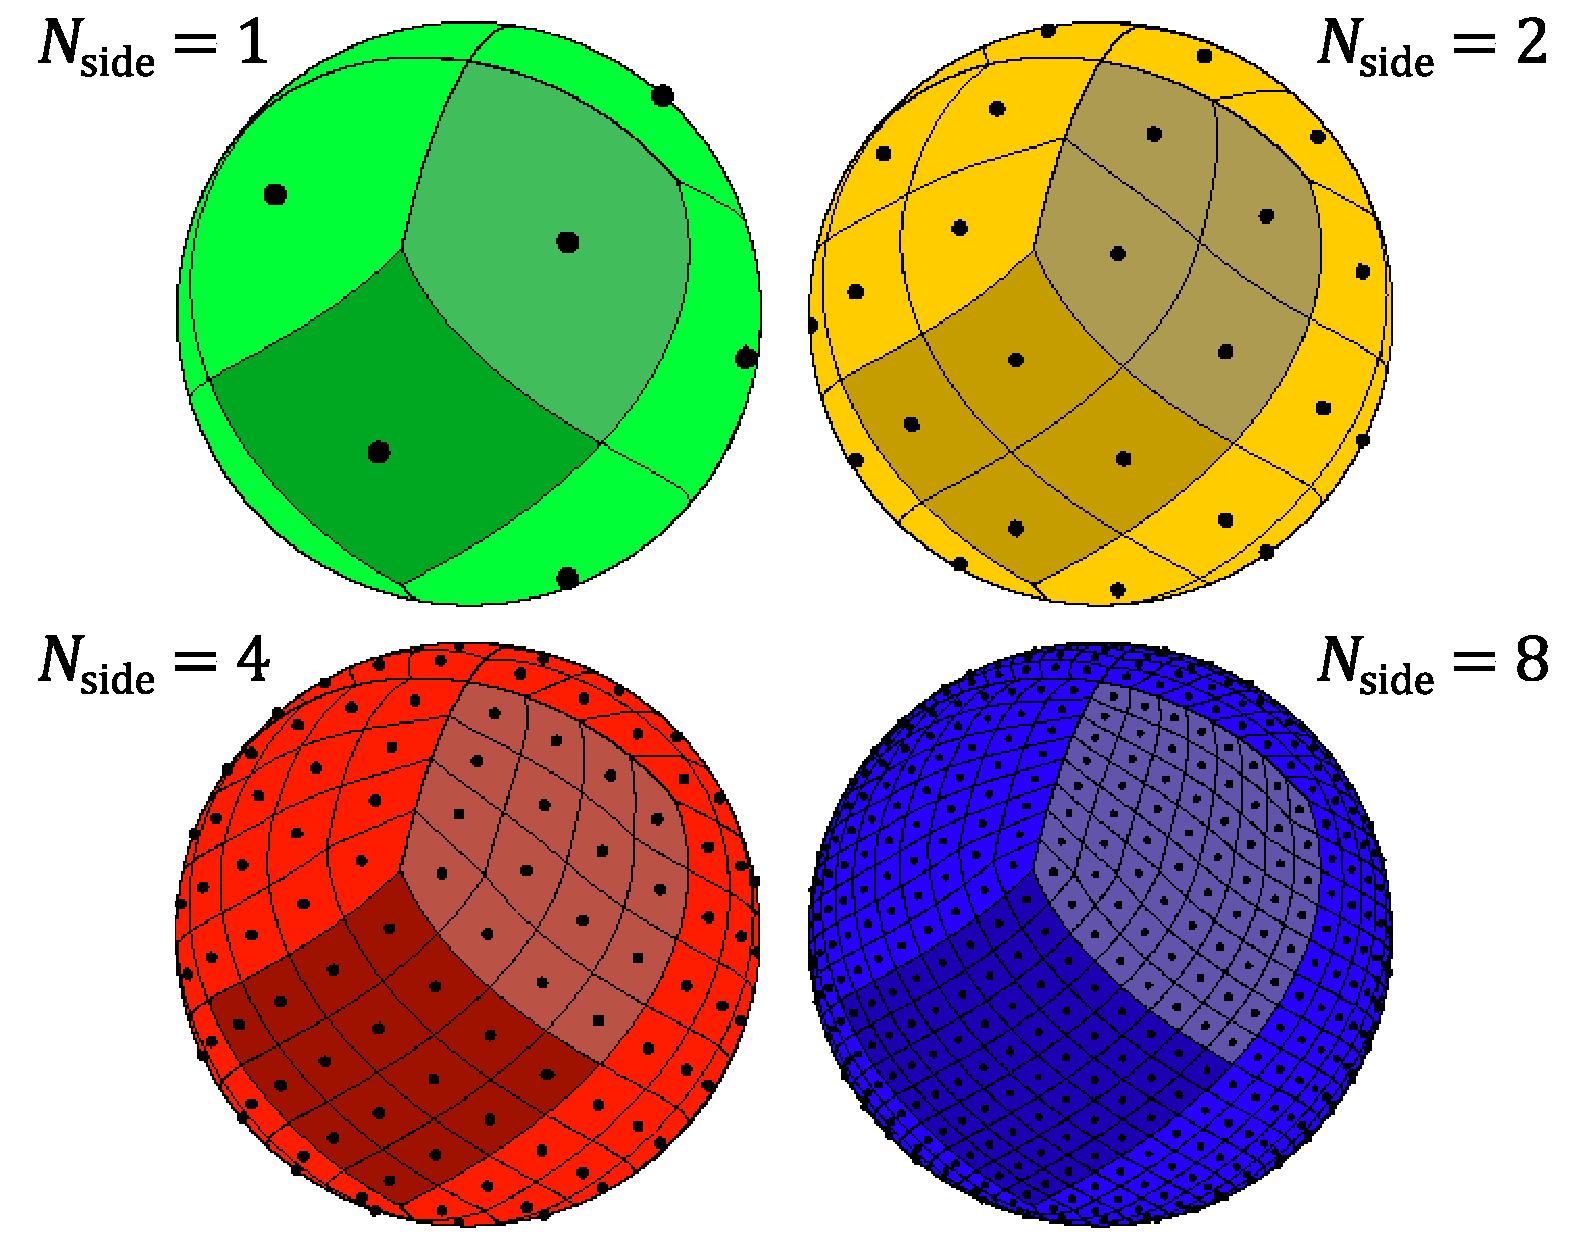
\includegraphics[width=0.7\linewidth]{images/healpix.pdf}
\end{center}
\caption[HEALPix partitions of a sphere]{HEALPix partitions of a sphere, of increasing order and $N_\text{side}$ resolution parameter. Note that as the resolution increases each pixel on the previous sphere is split into four on the new sphere, and $N_\text{side}$ is the number of pixels along the side of a base-resolution pixel (two of which are highlighted). Adapted (colourised) from Figure~4 of \citet{HEALPix}.
}
\label{fig:healpix}
\end{figure}

In addition to being a way to divide the sphere, each HEALPix pixel has a unique index from one of two different numbering schemes: either the ring (counting around each ring from the north to the south) or nested (based on the sub-pixel tree) system. Each scheme has its own advantages, ring-indexed grids are easier to apply spherical harmonics to while nested grids are easier to enter into hierarchical databases. Ultimately for astronomical sky maps the harmonics are less relevant and so nested grids are usually used, but conversion between the two is fairly straightforward.

HEALPix is used to provide localisation of sky probabilities for transient astronomical events, in the form of sky maps. Each point on the HEALPix grid is assigned a probability between 0 and 1 that the counterpart object is located within that pixel, and the whole sphere should sum to unity. Figure~\ref{fig:example_skymap} shows an example \gls{lvc} skymap, produced as part of the ``First Two Years'' simulations \citep{First2Years}.

\begin{figure}[p]
\begin{center}
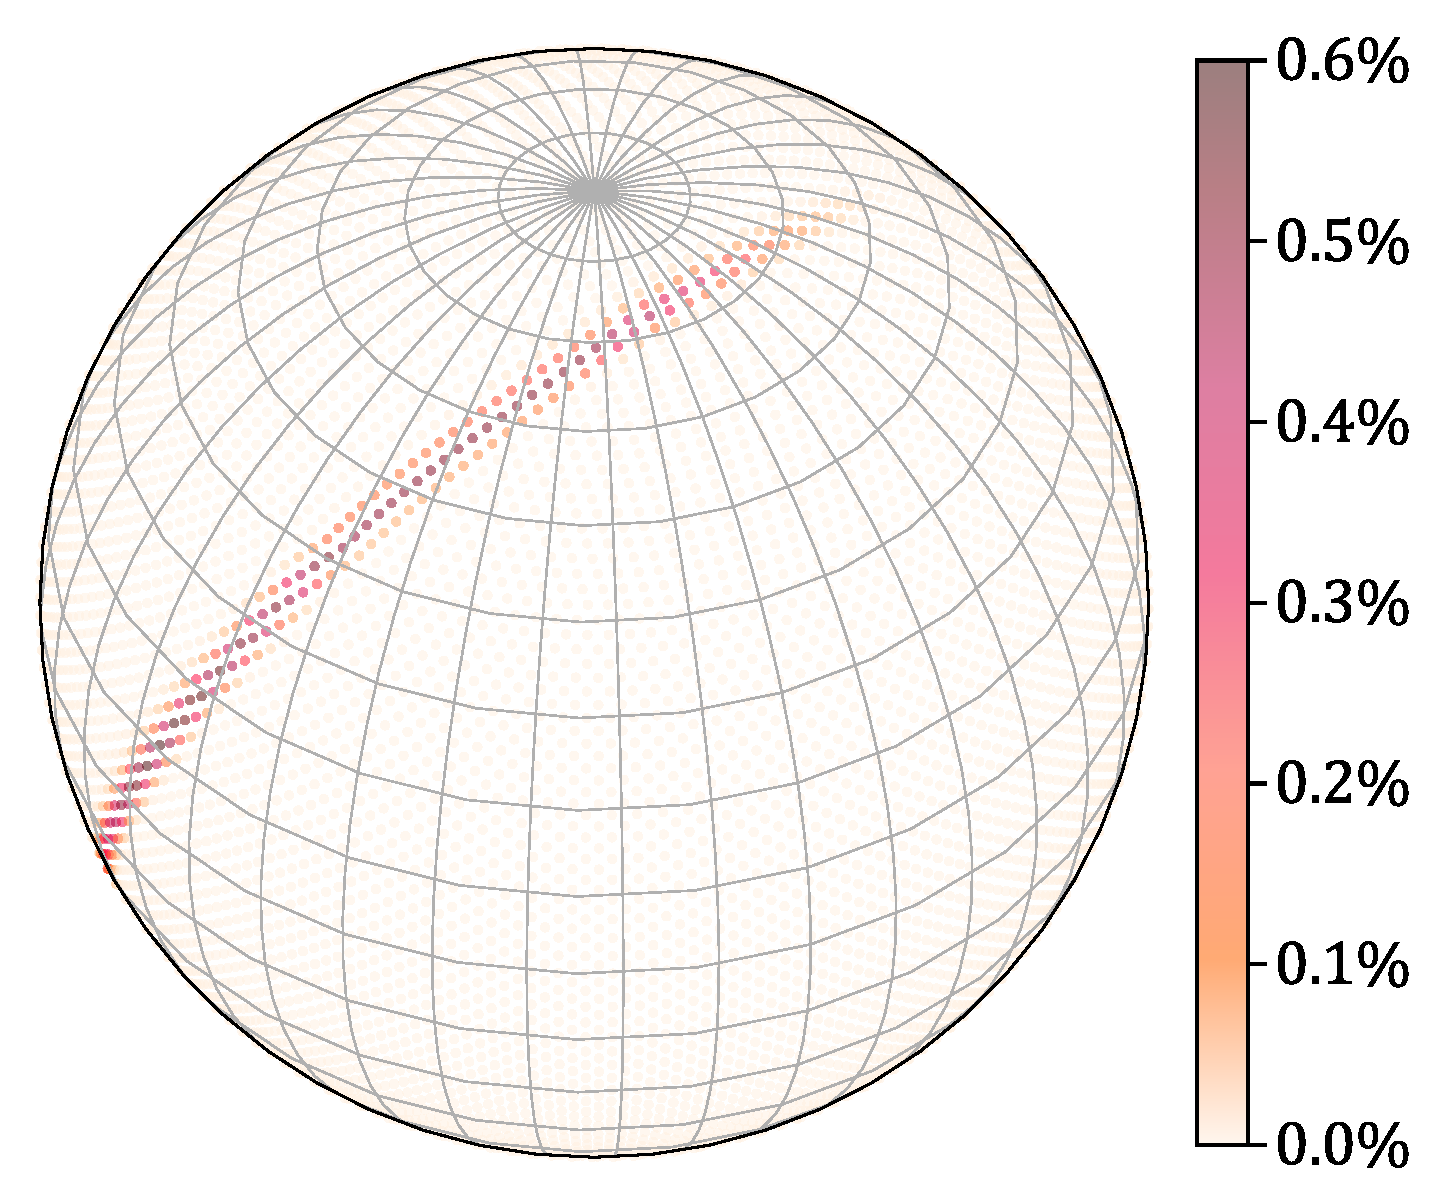
\includegraphics[width=\linewidth]{images/skymap_plot.pdf}
\end{center}
\caption[An example low-resolution skymap]{An example low-resolution gravitational wave skymap. The original skymap has been deliberately downgraded from $N_\text{side} = 256$ to $N_\text{side} = 32$ ($N_\text{pix} = 12288$) so that individual HEALPix pixels are visible. Each point is assigned a probability value as shown by the colour scale, which indicates the contained probability within that pixel.
}
\label{fig:example_skymap}
\end{figure}

\end{colsection}

% ~~~~~~~~~~~~~~~~~~~~

\subsection{Mapping sky maps to sky grids}
\label{sec:mapping_skymaps}
\begin{colsection}

When gravitational wave signals are detected the \gls{lvc} analysis pipelines create HEALPix sky maps to describe the sky localisation, and these are then distributed with the public VOEvent (see Section~\ref{sec:voevents}). GOTO-tile uses these skymaps to produce follow-up targets for \gls{goto}. This is done by mapping the sky maps onto the previously-defined all-sky grid used for the all-sky survey. As described previously in Section~\ref{sec:grids}, these grids are defined by a series of tiles covering the celestial sphere. GOTO-tile's task is to find all of the HEALPix points that fall within each tile, and then summing the probability values for each of these points gives the contained probability within the tile.

The first step to finding the probability contained within a tile is to define the edges of the tile in terms of celestial coordinates. This is done using the \code{get\_tile\_vertices} function within \pkg{gototile} written by Evert Rol. After that a polygon is defined that matches the tile area, and then using the \pkg{healpy} \code{query\_polygon} function the indices of the HEALPix points within each tile are found. This of course differs depending on the resolution required, and so is only calculated when applying a sky map with a defined $N_\text{side}$ to the previously-generated grid. Once it's found which HEALPix points are within a given tile it's easy to mask the skymap HEALPix array and sum the probability of these points, which gives the total contained probability within each tile.

Figure~\ref{fig:170817_tiles} shows an example of GOTO-tile applied to the sky map for the GW170817 event (\cite{GW170817}). The points within each tile were identified and summed in order to find the total contained probability within each tile. There is some redundancy due to the overlap between tiles, however this is typically negligible (the final GW170817 sky map used was notably smaller than usual LVC sky maps due to the coincident \textit{Fermi} localisation, which makes the overlaps more pronounced).

\begin{sidewaysfigure}[p]
\begin{center}
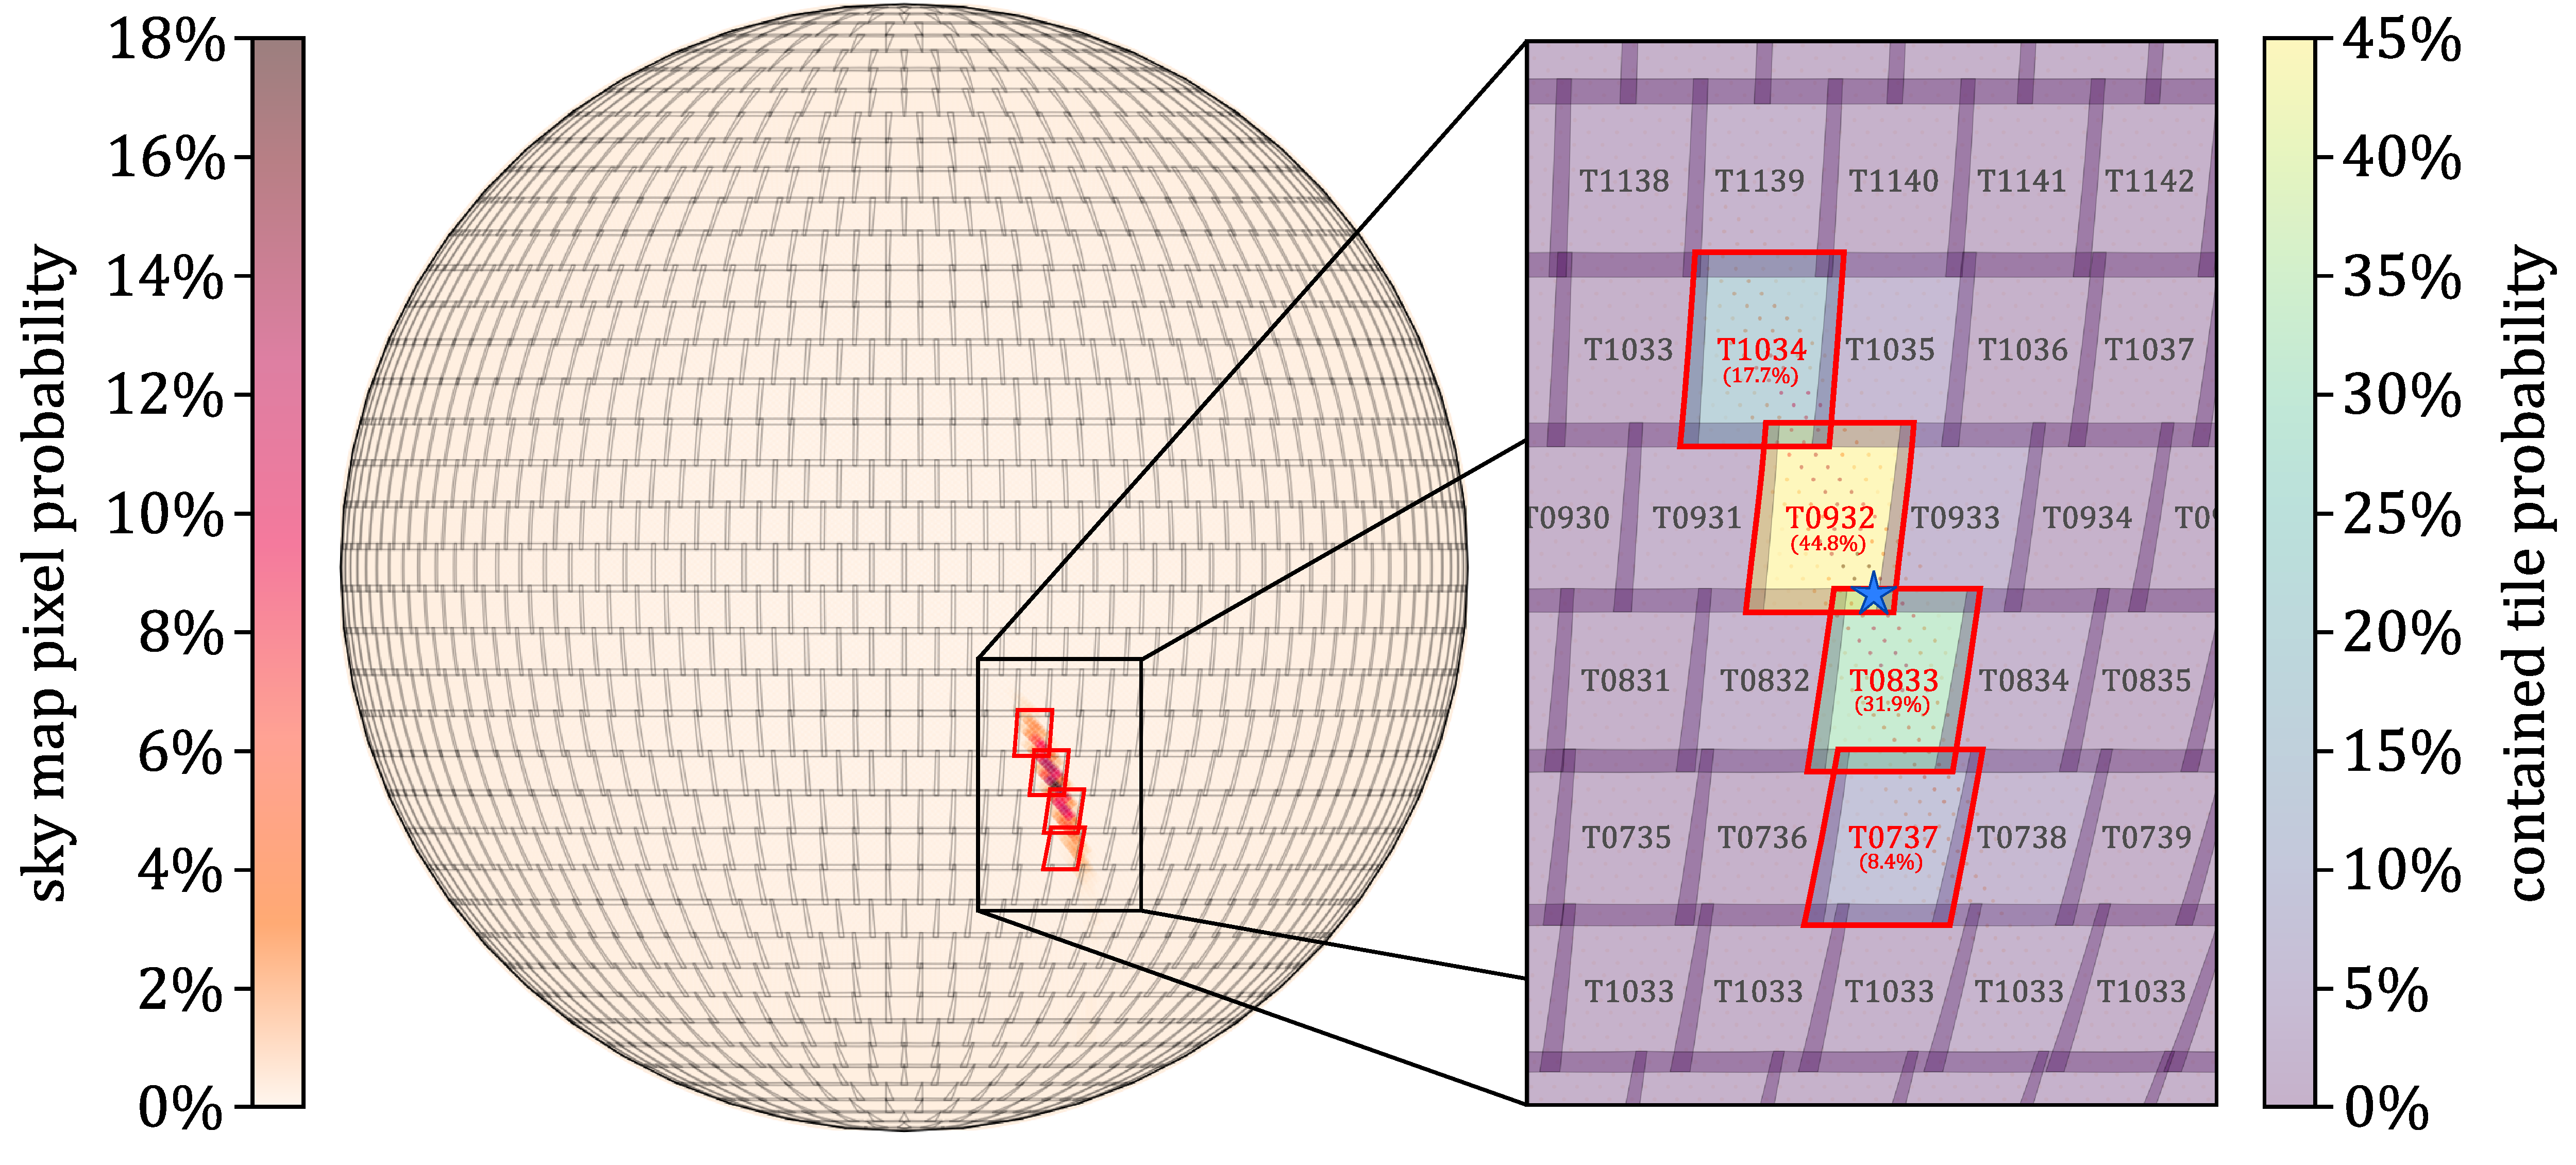
\includegraphics[width=\linewidth]{images/170817_tileplot.pdf}
\end{center}
\caption[Tile probabilities using GW170817]{Tile probabilities using the final sky map for GW170817 (\cite{GW170817}). The sphere shows the whole skymap for this event, with each pixel coloured by probability. Overlaid is the GOTO-4 sky grid, with tiles of \SI{3.7}{\degree} $\times$ \SI{4.9}{\degree} and overlap of $0.1$. The inset shows the tiles overlaid and coloured by their contained probability (the sum of all pixel within). The four tiles with contained probability of higher than 5\% are highlighted in red. The combined probability of these tiles adds to greater than 100\%, due to the overlapping regions being counted twice. The actual probability covered by the four tiles accounting for this is 92\%.
}
\label{fig:170817_tiles}
\end{sidewaysfigure}

\newpage

\end{colsection}

% ~~~~~~~~~~~~~~~~~~~~

\subsection{Creating sky maps for GRB events}
\label{sec:grb_skymaps}
\begin{colsection}

This system described in the previous sections works well for gravitational wave events using \gls{lvc} skymaps, and it has since ben expanded to other types of events. As part of the commissioning observations (\rtxt{see commissioning}) when the LIGO-Virgo detectors were down \gls{goto} also followed-up \gls{grb} events from the \textit{Fermi} satellite \gls{gbm}. 

\end{colsection}

% ~~~~~~~~~~~~~~~~~~~~

\end{colsection}

% ########################################

\newpage
\section{Alert processing with GOTO-alert}
\label{sec:gotoalert}
\begin{colsection}

% ~~~~~~~~~~~~~~~~~~~~

\begin{colsection}

WIP

\end{colsection}

% ~~~~~~~~~~~~~~~~~~~~

\subsection{The VOEvent schema}
\label{sec:voevents}
\begin{colsection}

WIP

\end{colsection}

% ~~~~~~~~~~~~~~~~~~~~

\subsection{Processing VOEvents}
\label{sec:alert_processing}
\begin{colsection}

WIP

\end{colsection}

% ~~~~~~~~~~~~~~~~~~~~

\end{colsection}

% ########################################

\newpage
\section{Observing with GOTO}
\label{sec:observing}
\begin{colsection}

% ~~~~~~~~~~~~~~~~~~~~

\begin{colsection}

WIP

\end{colsection}

% ~~~~~~~~~~~~~~~~~~~~

\subsection{Observing on the grid}
\label{sec:grid_observing}
\begin{colsection}

WIP

\end{colsection}

% ~~~~~~~~~~~~~~~~~~~~

\subsection{Alert follow-up}
\label{sec:alert_followup}
\begin{colsection}

WIP

\end{colsection}

% ~~~~~~~~~~~~~~~~~~~~

\subsection{Scheduler simulations}
\label{sec:simulations}
\begin{colsection}

WIP

\end{colsection}

% ~~~~~~~~~~~~~~~~~~~~

\subsection{Gravitational wave observations}
\label{sec:gw_followup}
\begin{colsection}

WIP

\end{colsection}

% ~~~~~~~~~~~~~~~~~~~~

\subsection{Other transient follow-up}
\label{sec:other_followup}
\begin{colsection}

WIP

\end{colsection}

% ~~~~~~~~~~~~~~~~~~~~

\end{colsection}

% ########################################
